% =============================================================
% fig_uq_pipeline.tex
% Cooperative aleatoric/epistemic uncertainty pipeline (Section 3.6-3.7)
% Compile standalone:  pdflatex fig_uq_pipeline.tex
% =============================================================
\documentclass[tikz, border=8pt]{standalone}
\usepackage{amsmath,amssymb}
\usetikzlibrary{arrows.meta, positioning, fit, backgrounds, calc}

% ---- Shared colour palette (kept identical across the architecture figures) ----
\definecolor{cInput}{HTML}{4477AA}    % blue    - input / backbone
\definecolor{cSpatial}{HTML}{8855AA}  % violet  - variance network
\definecolor{cGraph}{HTML}{EE9922}    % amber   - epistemic / SGLD
\definecolor{cTemporal}{HTML}{229988} % teal    - outputs
\definecolor{cOutput}{HTML}{EE6677}   % coral   - final uncertainty outputs
\definecolor{cMuted}{HTML}{999999}    % grey    - not yet integrated

\tikzset{
  font=\sffamily,
  block/.style={draw=black!70, rounded corners=3pt, line width=0.7pt,
    text width=3.8cm, align=center, font=\sffamily\small,
    minimum height=1.3cm, inner sep=5pt},
  inputblock/.style={block, fill=cInput!15, draw=cInput!75!black},
  varblock/.style={block, fill=cSpatial!15, draw=cSpatial!75!black},
  epiblock/.style={block, fill=cGraph!12, draw=cGraph!70!black, dashed,
    text=black!65},
  outbadge/.style={circle, draw=cTemporal!75!black, fill=cTemporal!15,
    minimum size=1.25cm, font=\sffamily\scriptsize, line width=0.7pt,
    align=center},
  outbadgemuted/.style={outbadge, draw=cMuted, dashed, fill=cMuted!10,
    text=black!55},
  flow/.style={-{Latex[length=2.6mm, width=1.9mm]}, line width=0.9pt, draw=black!70},
  mutedflow/.style={-{Latex[length=2mm, width=1.5mm]}, line width=0.6pt, draw=cMuted, dashed},
  steplabel/.style={font=\bfseries\scriptsize, text=black!70, align=left},
  statuslabel/.style={font=\scriptsize\itshape, align=center},
  donelabel/.style={statuslabel, text=cTemporal!60!black},
  progresslabel/.style={statuslabel, text=cSpatial!70!black},
  pendinglabel/.style={statuslabel, text=cMuted},
}

\begin{document}
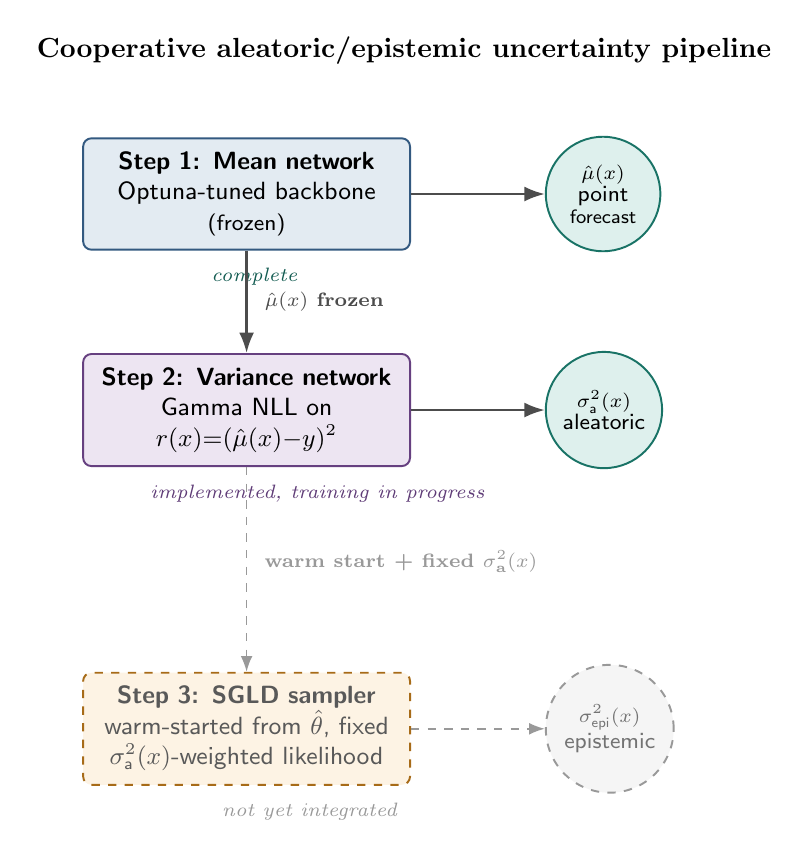
\begin{tikzpicture}[node distance=13mm]

  % ----------------------------------------------------------------
  % Step 1: mean network (already trained, frozen)
  % ----------------------------------------------------------------
  \node[inputblock] (mean)
    {\textbf{Step 1: Mean network}\\ Optuna-tuned backbone\\ \footnotesize (frozen)};
  \node[outbadge, right=17mm of mean] (muhat) {$\hat\mu(x)$\\ \footnotesize point\\ forecast};
  \node[donelabel, below=1mm of mean, xshift=1mm] {complete};

  \draw[flow] (mean) -- (muhat);

  % ----------------------------------------------------------------
  % Step 2: variance network (implemented, in progress)
  % ----------------------------------------------------------------
  \node[varblock, below=of mean] (var)
    {\textbf{Step 2: Variance network}\\ Gamma NLL on $r(x){=}(\hat\mu(x){-}y)^2$};
  \node[outbadge, right=17mm of var] (sigma_a) {$\sigma^2_\text{a}(x)$\\ \footnotesize aleatoric};
  \node[progresslabel, below=1mm of var, xshift=9mm] {implemented, training in progress};

  \draw[flow] (var) -- (sigma_a);
  \draw[flow] (mean.south) -- (var.north)
    node[steplabel, midway, right=1mm] {$\hat\mu(x)$ frozen};

  % ----------------------------------------------------------------
  % Step 3: epistemic sampler (not yet integrated)
  % ----------------------------------------------------------------
  \node[epiblock, below=26mm of var] (epi)
    {\textbf{Step 3: SGLD sampler}\\ warm-started from $\hat\theta$, fixed\\ $\sigma^2_\text{a}(x)$-weighted likelihood};
  \node[outbadgemuted, right=17mm of epi] (sigma_epi) {$\sigma^2_\text{epi}(x)$\\ \footnotesize epistemic};
  \node[pendinglabel, below=1mm of epi, xshift=8mm] {not yet integrated};

  \draw[mutedflow] (epi) -- (sigma_epi);
  \draw[mutedflow] (var.south) -- (epi.north)
    node[steplabel, midway, yshift=1mm, right=1mm, text=cMuted] {warm start + fixed $\sigma^2_\text{a}(x)$};

  % ----------------------------------------------------------------
  % Title
  % ----------------------------------------------------------------
  \node[font=\bfseries\normalsize, above=8mm of mean, xshift=20mm]
    {Cooperative aleatoric/epistemic uncertainty pipeline};

\end{tikzpicture}
\end{document}
